\documentclass[brazil]{beamer}
\usepackage{template}
\begin{document}

% Slide de Título
{
    % Salva o template original do headline
    \let\oldheadline\beamertemplateheadline
    % Remove a barra superior
    \setbeamertemplate{headline}{}
    \begin{frame}
        \titlepage
    \end{frame}

    % Restaura o headline para o restante do documento
    \let\beamertemplateheadline\oldheadline
}

%================================================
\begin{frame}{Sumário}
    \tableofcontents
\end{frame}

%================================================
\section{Introdução}
\begin{frame}{Uma visão do MAESTRO}
    \hspace{0.5cm}Para o surgimento de \textbf{ideias e propostas} de soluções de problemas 
    são necessárias \textbf{discussões} que possam \textbf{enriquecer} nossa visão tanto de forma mais 
    abrangente quanto especifica do nosso problema. Como consequência, uma sequencia 
    de \textbf{perguntas cruciais} com diferentes pontos de vista são levantadas e podem até 
    mesmo ser a nossa solução.
\end{frame}

\begin{frame}{Pontos fracos discutidos do MAESTRO}
    \begin{itemize}
        \item Baseado em pacotes, fixa e não dinâmica.
        \item Orquestração muito baixa ou zero.
    \end{itemize}
\end{frame}

% \begin{frame}{O que poderia ser melhorado?}
%     \begin{itemize}
%         \item O que faria 
%         \item Orquestração muito baixa ou zero.
%     \end{itemize}
% \end{frame}

%================================================
\section{Ideias e propostas}
\begin{frame}{O inicio de tudo, Pacote-F}
    \hspace{0.5cm}Com a introdução do Pacote-F, foram implementadas alterações interessantes 
    e promissoras, onde foi necessário utilizar \textbf{mais de uma gNB} e em \textbf{diferentes slices}. 
    Isso permitiu não somente subir uma infraestrutura de rede, mas a possibilidade de subir 
    \textbf{varias infraestruturas} em um \textbf{único deploy}.
\end{frame}

\begin{frame}{O que implicaria um pacote mais dinâmico?}
    \hspace{0.5cm}Um pacote mais dinâmico não permitiria somente uma maior poder de flexibilidade ao 
    usuário(que foi planejado inicialmente), mas também habilitaria a possibilidade de customizar 
    e entregar músicos ao maestro. Afinal, o que é uma orquestra sem músicos?
\end{frame}

\begin{frame}{Tudo que temos em um só, Pacote-Z}
    \hspace{0.5cm}Projetado para \textbf{entregar tudo} que temos em um único pacote, \textbf{o primeiro  e 
    talvez ultimo} "\textit{pacoteless}". Atualmente, no nosso laboratório tem diversos projetos e focos enriquecedores 
    tanto na parte mais física com antenas até de a transição de funções de para nuvem(CFVs). O MAESTRO seria a 
    oportunidade de juntar tudo que um usuário poderia querer de uma fácil, rápida e escalável para futura 
    orquestração massiva englobando varias areas como cidades inteligentes.
\end{frame}

\begin{frame}{O que é pensado para a transição inicial}
    \begin{itemize}
        \item Único pacote(Z) para customizações mais especificas.
        \item Escolha de arquiteturas: OAI, open5GS e etc.
        \item Escolha de deploy: BareMetal, Kubernets e etc.
        \item Escolha de quantidade de gNBs com slice aplicado.
        \item Escolha de quantidade de serviços e quais deles.
        \item Desagregação do core com escolha de arquitetura e deploy(CNF).
    \end{itemize}
\end{frame}

\begin{frame}{Futuro mais dinamico e orquestrado}
    \begin{itemize}
        \item Areas inteligentes.
        \item Orquestração de infraestrutura por areas.
        \item Monitoramento inteligente com cidades inteligentes.
    \end{itemize}
\end{frame}

%================================================
\section{Resultados}
\begin{frame}{Objetivos alcançados atualmente no pacote-Z}
    \begin{itemize}
        \item Escolha de arquiteturas: OAI, open5GS e etc.
        \item Escolha de quantidade de gNBs com slice aplicado(apenas com open5GS).
        \item \textit{Deploy} de componentes de forma dinâmica.
    \end{itemize}
\end{frame}

\begin{frame}{Maquinas e Serviços}
\begin{figure}
    \centering
    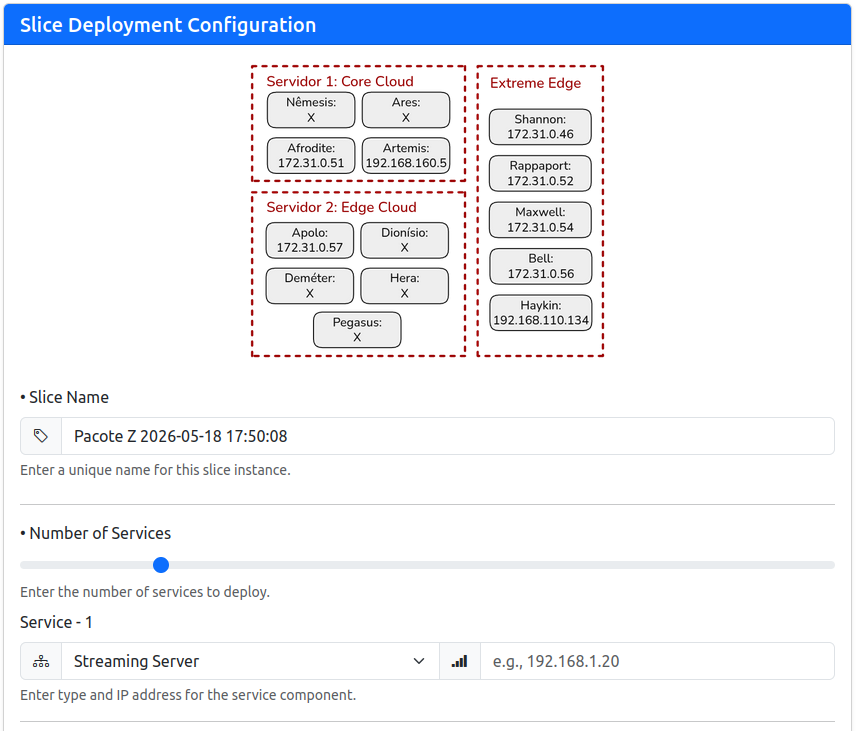
\includegraphics[width=0.7\linewidth]{etc/ms.png}
    %\caption{Todas as maquinas e serviços}
    \label{fig:ms}
\end{figure}
\end{frame}

\begin{frame}{Core e gNBs}
\begin{figure}
    \centering
    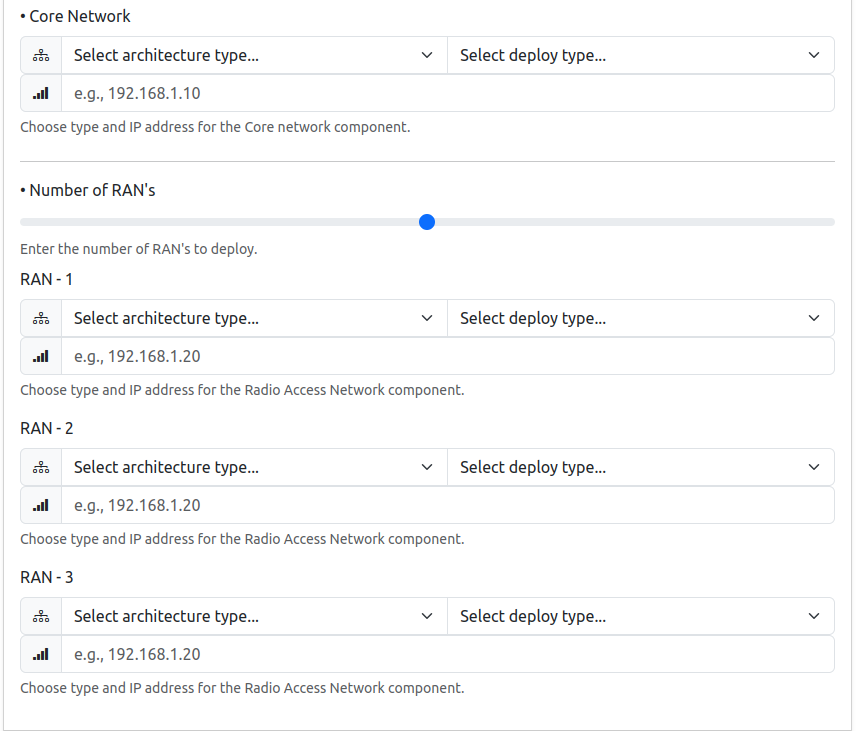
\includegraphics[width=0.7\linewidth]{etc/cb.png}
    %\caption{Core e gNBs}
    \label{fig:cb}
\end{figure}
\end{frame}

\begin{frame}{Problemas encontrados}
    \hspace{0.5cm}Devido ao estado atual do MAESTRO, que é integrado o comissionamento 
    por pacotes, ele não permite uma fácil seleção do usuário de componentes no frontend 
    de forma dinâmica. É necessário alterar ou permitir o comissionamento de componentes 
    individuais, no qual foi resolvido parcialmente. 
\end{frame}

%================================================
\section{Conclusão}
\begin{frame}{Conclusão}
    \hspace{0.5cm}Foram encontradas soluções não apenas de deixar o MAESTRO mais customizável, 
    mas de deixa-lo mais dinâmico, modular, flexível e pratico. Habilitando aplicações futuras 
    de orquestração.
\end{frame}

% %================================================
% \section{Referências}
% %\bibitem{Ex2} citação Disponível em: {\url{link}}. Acesso em: .
% \begin{frame}[allowframebreaks]
% \small
% \begin{thebibliography}{99}
% \bibitem{flexric2}
% Mosaic5g. Flexric - br-flexric - GitLab. Disponível em: <{\url{https://gitlab.eurecom.fr/mosaic5g/flexric/-/tree/br-flexric}}>. Acesso em: 19 nov. 2025.
% \end{thebibliography}
% \end{frame}

%================================================
\section{Agradecimentos}
\begin{frame}
\centering
O presente trabalho foi realizado com apoio do CNPq, Conselho Nacional de Desenvolvimento Científico e Tecnológico – Brasil
\end{frame}
\end{document}
